\documentclass{beamer}
\usetheme{metropolis}
\usepackage{graphicx}
\usepackage{subfig}
\usepackage{tcolorbox}
\title{Algebra-Based Physics: Electricity, Magnetism, and Modern Physics (PHYS135B): Unit 4}
\author{Jordan Hanson}
\institute{Whittier College Department of Physics and Astronomy}

\begin{document}
\maketitle

\section{Summary}

\begin{frame}{Summary}
\begin{enumerate}
\item Magnetic induction - \textbf{Chapters 23.1 - 23.5, 23.7, 23.9}
\begin{itemize}
\item Induced EMF and magnetic flux
\item Faraday's Law
\item Motional EMF, generators, and transformers
\end{itemize}
\item AC circuits - \textbf{Chapters 23.9 - 23.12}
\begin{itemize}
\item Inductors
\item RL circuits
\item RLC circuits
\end{itemize}
\end{enumerate}
\end{frame}

\section{Magnetic induction}

\begin{frame}{Magnetic induction}
\small
\textbf{\alert{First set of observations:}} a \textit{moving} magnet can induce an emf in a coil of wire.  The induced current polarity depends on (a) magnet polarity and (b) direction of magnet velocity.  The induced current magnitude 
\begin{figure}
\centering
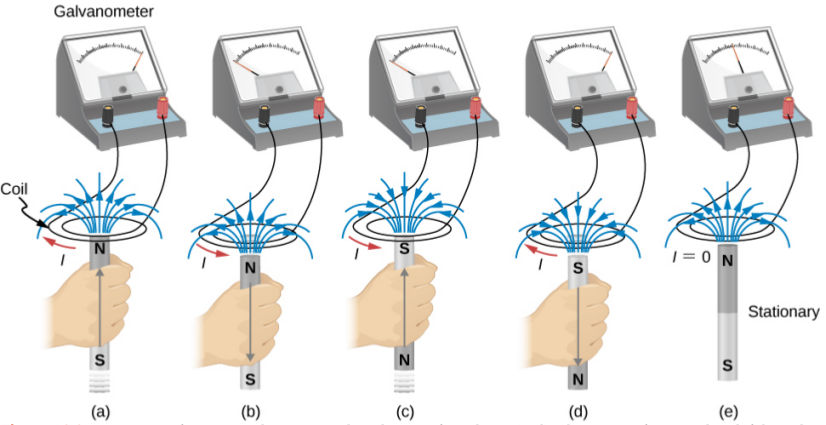
\includegraphics[width=0.8\textwidth]{figures/farad.png}
\caption{\label{fig:farad1} Observations of magnetic induction.}
\end{figure}
\end{frame}

\begin{frame}{Magnetic induction}
\small
\textbf{\alert{Second set of observations:}} a \textit{changing} current in a loop can induce an emf in another loop.  The induced current polarity depends on (a) inducing current polarity and (b) whether the inducing current is increasing or descreasing.
\begin{figure}
\centering
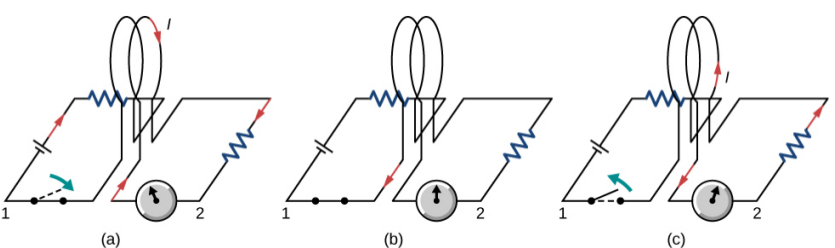
\includegraphics[width=0.8\textwidth]{figures/farad2.png}
\caption{\label{fig:farad2} Observations of magnetic induction.}
\end{figure}
\end{frame}

\begin{frame}{Magnetic induction}
\small
\textbf{\alert{Third observation:}} a \textit{changing} loop area in a magnetic field induces an emf, and current.  The induced current polarity depends on whether the loop area is (a) increasing or (b) descreasing.  The current magnitude depends on how quickly the area is changing.
\begin{figure}
\centering
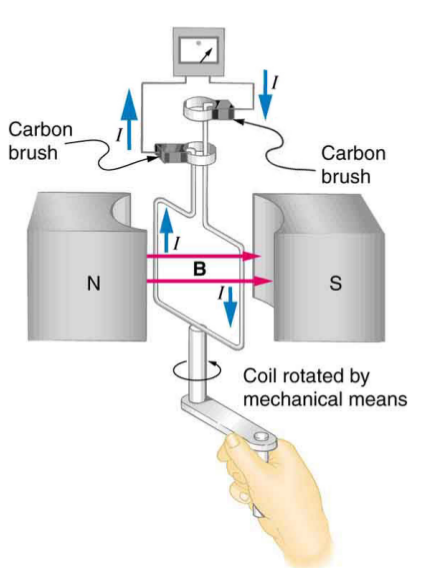
\includegraphics[width=0.3\textwidth]{figures/motorz.png}
\caption{\label{fig:motorz} Observations of magnetic induction.}
\end{figure}
\end{frame}

\begin{frame}{Magnetic induction}
Video summary of magnetic induction: \\
\url{https://youtu.be/pQp6bmJPU_0}
\begin{itemize}
\item Magnet inducing current in loop of wire
\item Solenoids inducing current in adjacent solenoids
\item Magnetic flux
\item Faraday's Law
\item Lenz's Law
\end{itemize}
\end{frame}

\begin{frame}{Magnetic induction}
\small
\textbf{\alert{Magnetic flux}} is the dot-product of the area vector and the magnetic field through loops of wire with area $A$.
\begin{columns}[T]
\begin{column}{0.5\textwidth}
\begin{figure}
\centering
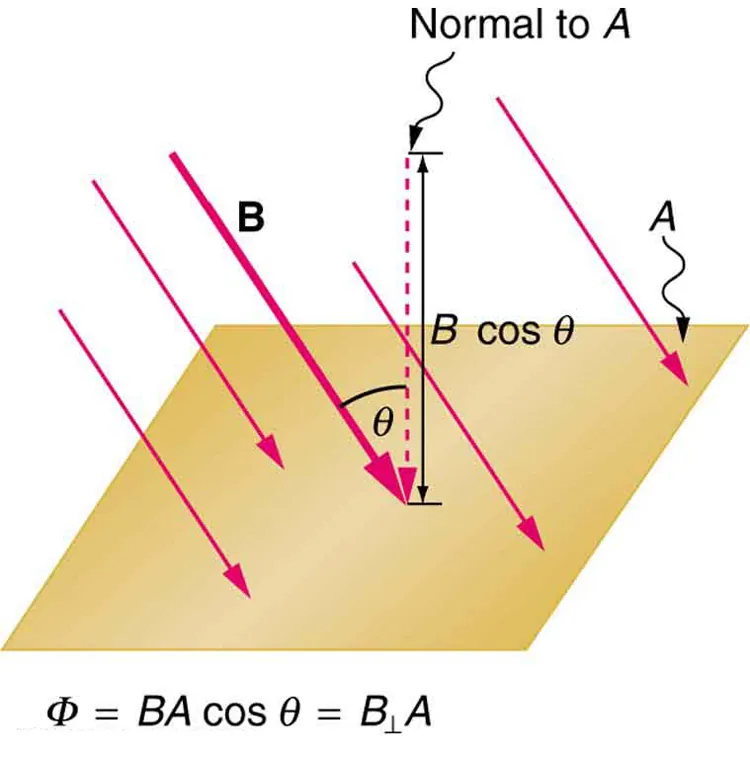
\includegraphics[width=0.95\textwidth]{figures/flux.png}
\caption{\label{fig:farad3} The \textbf{area vector} is \textit{normal} to the loop area.}
\end{figure}
\end{column}
\begin{column}{0.5\textwidth}
\vspace{0.5cm}
The \textbf{area vector} has a magnitude $A$, the area of the loop.  The direction of the area vector is \textit{normal} to the area of the loop.
\begin{equation}
\vec{A} = A \hat{n}
\end{equation}
The magnetic flux, $\Phi$, is therefore
\begin{equation}
\Phi = \vec{B} \cdot \vec{A}
\end{equation}
\end{column}
\end{columns}
\end{frame}

\section{Faraday's Law}

\begin{frame}{Faraday's Law}
\begin{tcolorbox}[colback=white,colframe=black!40!black,title=Faraday's Law]
\alert{Let the product of the magnetic field and the vector area be the magnetic flux: $\Phi = \vec{B} \cdot \vec{A}$.  The induced emf $\epsilon$ in $N$ turns of a conductor will be
\begin{equation}
\epsilon = - \frac{\Delta\Phi}{\Delta t}
\label{eq:farad}
\end{equation}
The induced current from $\epsilon$ will create a new B-field that opposes changes in $\Phi$.}
\end{tcolorbox}
\textit{The unit of magnetic flux is the Weber, or 1 Wb = 1 T m$^2$.}
\end{frame}

\begin{frame}{Faraday's Law}
\small
\begin{figure}
\centering
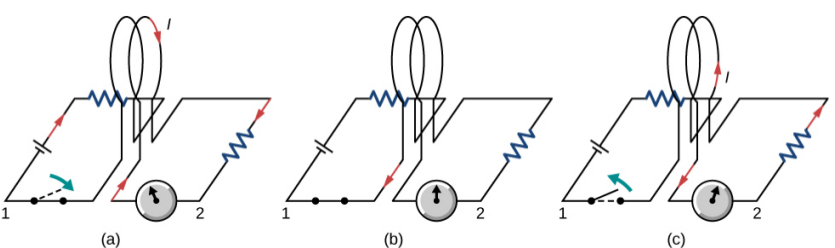
\includegraphics[width=0.7\textwidth]{figures/farad2.png}
\caption{\label{fig:loop1} A pickup coil system.}
\end{figure}
Suppose the switch in Fig. \ref{fig:loop1} (a) is closed, inducing a current $I$ in the right-hand loop.  The B-field directions at the centers of the left and right loops are
\begin{itemize}
\item A: Right and left, respectively
\item B: Light and right, respectively
\item C: Both to the right
\item D: Both to the left
\end{itemize}
\end{frame}

\begin{frame}{Faraday's Law}
\small
\begin{figure}
\centering
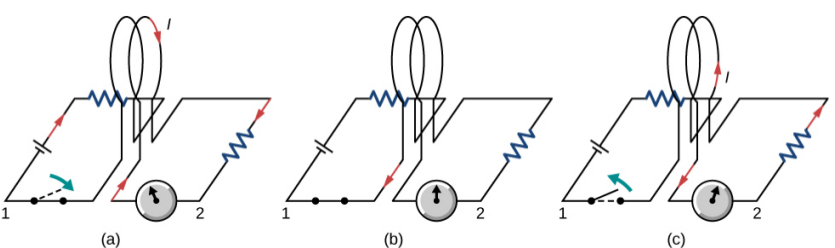
\includegraphics[width=0.7\textwidth]{figures/farad2.png}
\caption{\label{fig:loop2} A pickup coil system.}
\end{figure}
Suppose the switch in Fig. \ref{fig:loop1} (b) remains closed, and no induced current is observed.  This is because
\begin{itemize}
\item A: The magnetic flux is zero
\item B: The inducing current is zero
\item C: The magnetic flux is not changing
\item D: The loop area is zero
\end{itemize}
\end{frame}

\begin{frame}{Faraday's Law}
\small
\begin{figure}
\centering
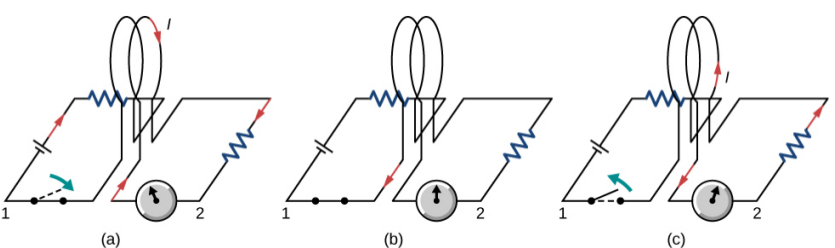
\includegraphics[width=0.7\textwidth]{figures/farad2.png}
\caption{\label{fig:loop3} A pickup coil system.}
\end{figure}
Suppose the switch in Fig. \ref{fig:loop1} (b) remains closed, and no induced current is observed.  This is because
\begin{itemize}
\item A: The magnetic flux is zero
\item B: The inducing current is zero
\item C: The magnetic flux is not changing
\item D: The loop area is zero
\end{itemize}
\end{frame}


\begin{frame}{Faraday's Law}
\small
\begin{figure}
\centering
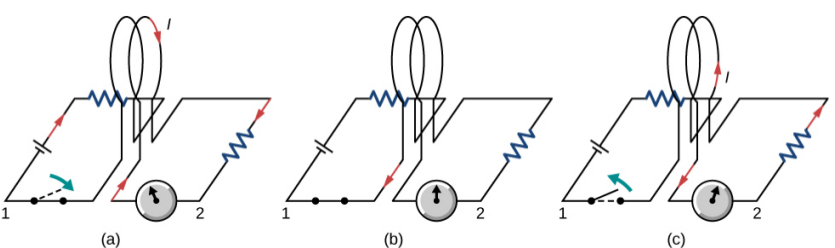
\includegraphics[width=0.7\textwidth]{figures/farad2.png}
\caption{\label{fig:loop4} A pickup coil system.}
\end{figure}
Suppose the switch in Fig. \ref{fig:loop1} (c) is opened.  The induced current in Fig. \ref{fig:loop1} is in the opposite direction of Fig. \ref{fig:loop1} (c) because
\begin{itemize}
\item A: The magnetic field from the right loop decreased
\item B: The magnetic field from the left loop increased
\item C: The magnetic field from the left loop is constant
\item D: The magnetic field from the left loop decreased
\end{itemize}
\end{frame}

\begin{frame}{Faraday's Law}
\small
\textbf{Group board problem:} \\ \vspace{0.5cm}
A magnetic field B passes orthogonally through a circular coil of radius $r = 0.05$ m and $N = 100$ turns.  The field magnitude decreases linearly according to
\begin{equation}
B(t) = B_0 - a t
\end{equation}
with $B_0 = 0.015$ T and $a = 0.01$ T s$^{-1}$.  (a) Calculate the magnitude of the emf induced in the coil at the times $t_0 = 0$, and $t_2 = 1.0$ second. (b) Determine the current in the coil if the resistance is 1 $\Omega$. \\ \vspace{0.5cm}
Sketch this system, and indicate both the direction of the instantaneous B-field, and the direction of current.
\end{frame}

\begin{frame}{Faraday's Law - PhET Activity}
\small
Brief simulation of Faraday's Law, and Lenz's Law: \\ \vspace{0.5cm}
\footnotesize
\url{https://phet.colorado.edu/en/simulations/faradays-law}
\small
\begin{enumerate}
\item Learn to control the position and orientation of the bar magnet.
\item Activate the voltmeter in parallel with the light bulb.
\item Use the coil with four loops of wire.
\item Produce the following results:
\begin{itemize}
\item A positve voltage from a moving bar magnet
\item A negative voltage from a moving bar magnet
\item A positive voltage from switching the bar magnet polarity
\item A negative voltage from switching the bar magnet polarity
\end{itemize}
\item Is your voltage positive or negative when you are increasing $\Phi$?  How do you \textit{decrease} $\Phi$?
\end{enumerate}
\end{frame}

\section{Motional EMF, Generators, and Transformers}

\begin{frame}{Motional EMF, Generators, and Transformers}
\small
\begin{figure}
\centering
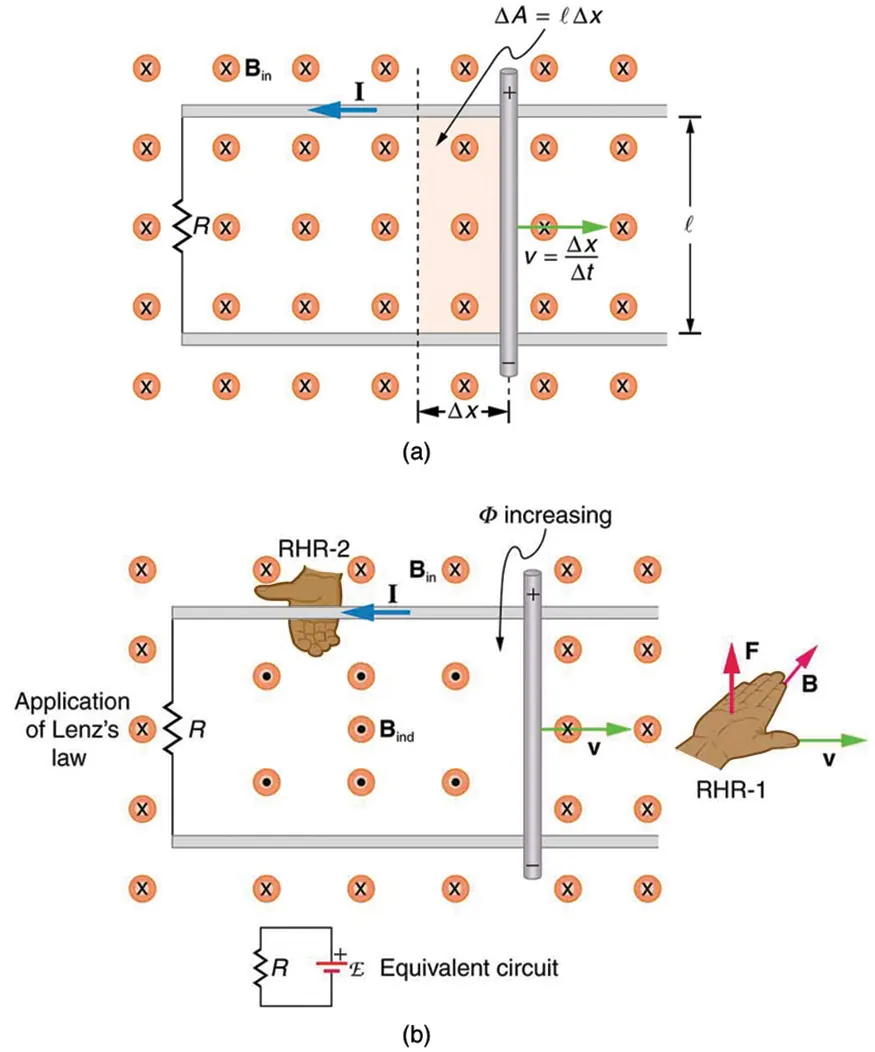
\includegraphics[width=0.44\textwidth,trim=4cm 20cm 4cm 0cm,clip=true]{figures/motion_emf.png}
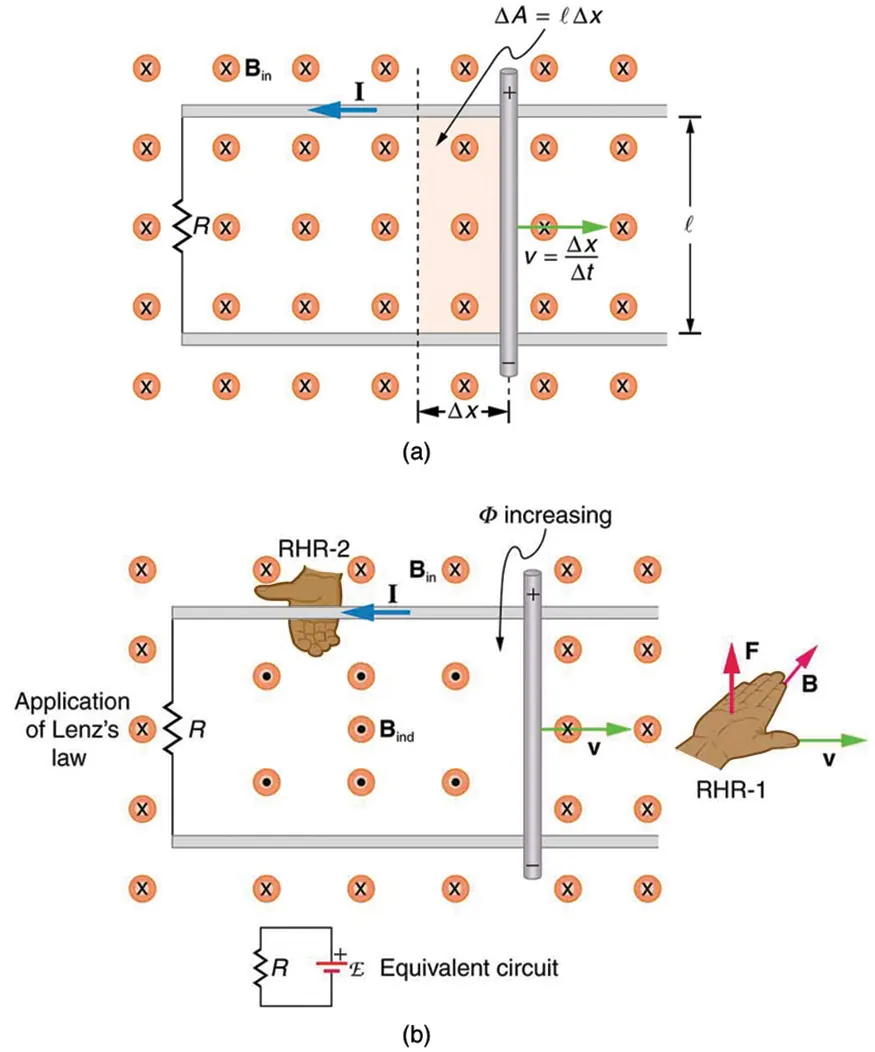
\includegraphics[width=0.54\textwidth,trim=0cm 0cm 0cm 18cm,clip=true]{figures/motion_emf.png}
\caption{\label{fig:motion_emf1} Motional emf in a loop with changing area.}
\end{figure}
\footnotesize
\textbf{\alert{Group board problems:}}
\begin{enumerate}
\item Show that \textit{power} is $P = \vec{F} \cdot \vec{v}$ when acceleration is constant.
\item Show that the emf is $\epsilon = B l v$, where $l$ is the length of the rod.
\item Show that power generated, $P = I^2 R = \epsilon/R$, is equal to power injected.
\end{enumerate}
\end{frame}

\begin{frame}{Motional EMF, Generators, and Transformers}
How do we use Faraday's Law to induce power in a generator?  Start with Faraday's Law:
\begin{equation}
\epsilon = - N\frac{\Delta \Phi}{\Delta t}
\end{equation}
The flux $\Phi$ depends on time:
\begin{equation}
\Phi = \vec{B} \cdot \vec{A}(t) = BA\cos(\theta(t))
\end{equation}
Let the \textit{angular velocity} be constant: $\theta = \omega t$.  Then we have
\begin{equation}
\Phi  = BA\cos(\omega t)
\end{equation}
Thus the emf (with $N$ loops) is (...calculus...)
\begin{equation}
\epsilon = N\omega BA \sin(\omega t) = \epsilon_0 \sin(\omega t)
\end{equation}
\end{frame}

\begin{frame}{Motional EMF, Generators, and Transformers}
\footnotesize
\begin{figure}
\centering
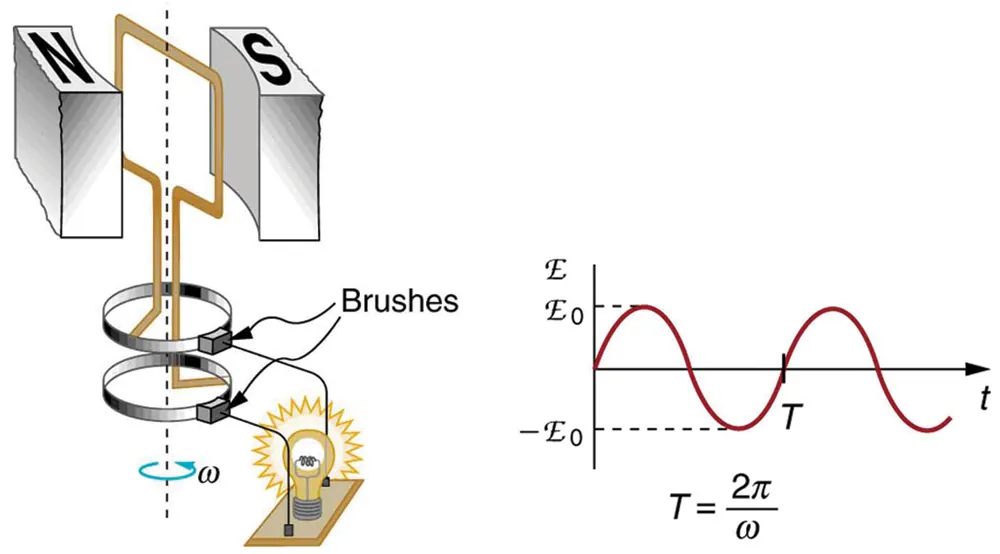
\includegraphics[width=0.65\textwidth]{figures/generator_1.png}
\caption{\label{fig:motion_emf2} (Left) The AC generator with brushes generates an AC voltage. (Right) This is a diagram of the AC voltage.}
\end{figure}
\begin{itemize}
\item Amplitude: $\epsilon_0$, the maximum value of the AC signal. Units: Volts.
\item Period: $T = 2\pi/\omega$, the time to complete one AC cycle.  Units: seconds.
\item Frequency: $f = 1/T$, the number of cycles per second.  Units: Hertz.
\end{itemize}
\end{frame}

\begin{frame}{Motional EMF, Generators, and Transformers}
\footnotesize
\begin{figure}
\centering
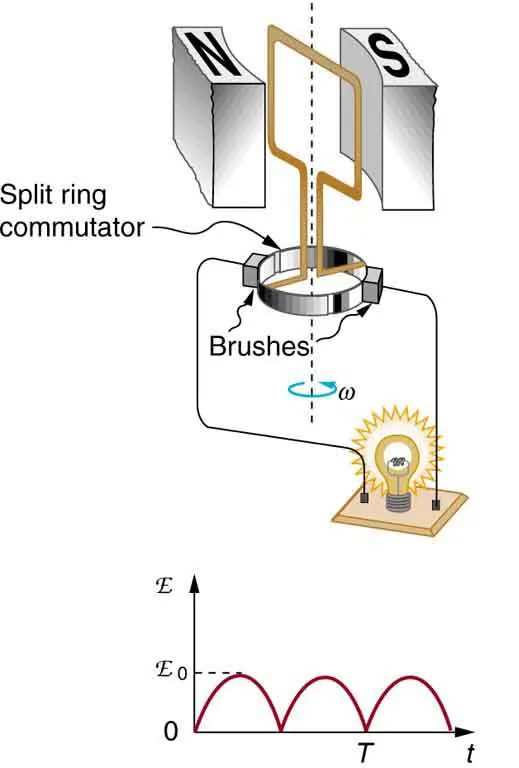
\includegraphics[width=0.35\textwidth,trim=0cm 8cm 0cm 0cm,clip=true]{figures/generator_2.png}
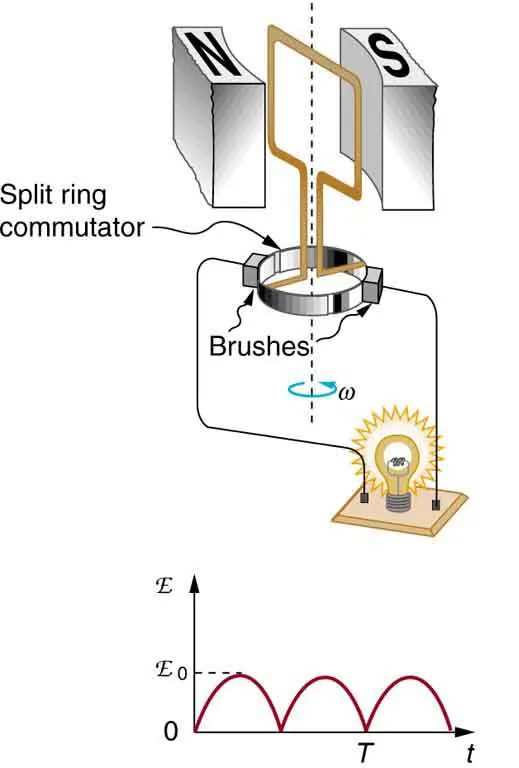
\includegraphics[width=0.5\textwidth,trim=0cm 0cm 0cm 20cm,clip=true]{figures/generator_2.png}
\caption{\label{fig:motion_emf3} (Left) The AC generator with brushes and \textit{commutator} generates pulsed DC. (Right) This is a diagram of the signal.}
\end{figure}
\begin{itemize}
\item Amplitude: $\epsilon_0$, the maximum value of the AC signal. Units: Volts.
\item Period: $T = 2\pi/\omega$, the time to complete one AC cycle.  Units: seconds.
\item Frequency: $f = 1/T$, the number of cycles per second.  Units: Hertz.
\end{itemize}
\end{frame}

\begin{frame}{Motional EMF, Generators, and Transformers}
Equation \ref{eq:gen} is a basic model for the emf from a generator.
\begin{equation}
\epsilon = N\omega BA \sin(\omega t) = \epsilon_0 \sin(\omega t) \label{eq:gen}
\end{equation}
Which of the following would increase the \textit{amplitude} of the emf?
\begin{itemize}
\item A: Turning the shaft more slowly
\item B: Turning the shaft more quickly
\item C: Decreasing the B-field
\item D: Increasing $N$
\end{itemize}
\end{frame}

\begin{frame}{Motional EMF, Generators, and Transformers}
Equation \ref{eq:gen2} is a basic model for the emf from a generator.
\begin{equation}
\epsilon = N\omega BA \sin(\omega t) = \epsilon_0 \sin(\omega t) \label{eq:gen2}
\end{equation}
Which of the following would increase the \textit{frequency} of the emf?
\begin{itemize}
\item A: Turning the shaft more slowly
\item B: Turning the shaft more quickly
\item C: Decreasing the B-field
\item D: Increasing $N$
\end{itemize}
\end{frame}

\begin{frame}{Motional EMF, Generators, and Transformers}
Equation \ref{eq:gen3} is a basic model for the emf from a generator.
\begin{equation}
\epsilon = N\omega BA \sin(\omega t) = \epsilon_0 \sin(\omega t) \label{eq:gen3}
\end{equation}
\textbf{Group exercise:} Suppose an AC generator rotates at 200 rpm, in a B-field with 0.1 T, and has 100 loops with radius 5 cm.  (a) What is the peak voltage this generator will produce? (b) If the generator powers a system with resistance of 1k$\Omega$, what will be the peak current?
\end{frame}

\section{PhET: Motional EMF, Generators, and Transformers}

\begin{frame}{PhET: AC Power generator}
\footnotesize
Link to the (CheerpJ) simulation: \\ \vspace{0.2cm}
\url{https://phet.colorado.edu/en/simulation/generator}
\begin{enumerate}
\item Set the water rate such that the meter reads 10 rotations per minute (rpm).
\item Choose the voltage meter under the pickup coil menu.
\item Under loops, choose 1 loop, and under area, leave it at 50\%.
\item Choose show field meter in the upper right, and place the tool in the loop center.
\item On the same graph, plot the average B-field and voltage versus time.  What is the period and amplitude of your signal?  Use the left y-axis for B-field units, and the right y-axis for voltage units.
\item Create the same graph for $N = 3$ loops.
\item Create the same graph for $N = 1$ loop, but for 20 rpm.
\end{enumerate}
\textit{Hint: you know the rpm of the magnet, so you know how much time corresponds to one rotation.}
\end{frame}

\begin{frame}{Motional EMF, Generators, and Transformers}
\small
\begin{figure}
\centering
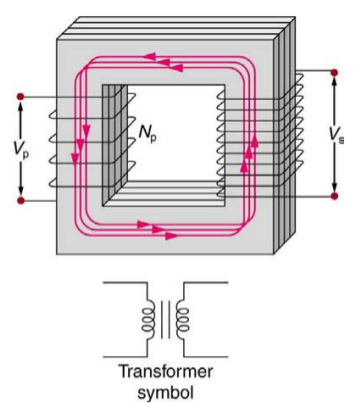
\includegraphics[width=0.45\textwidth,trim=0cm 5cm 0cm 0cm,clip=true]{figures/transformer.png}
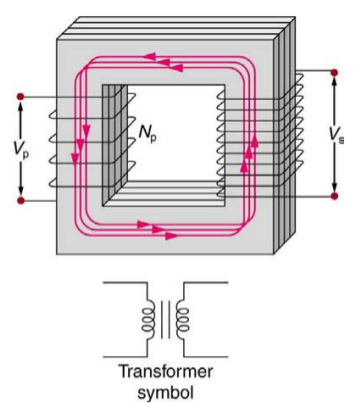
\includegraphics[width=0.25\textwidth,trim=3.0cm 0cm 4cm 10cm,clip=true]{figures/transformer.png}
\caption{\label{fig:trans1} A \textit{transformer} uses Faraday's law to change voltages in AC-generated systems.}
\end{figure}
The magnetizable core (gray) creates a loop in the B-field that passes through the left and right coils.  Use Faraday's law to show that
\begin{equation}
\frac{V_L}{V_R} = \frac{N_L}{N_R}
\end{equation}
\end{frame}

\begin{frame}{Motional EMF, Generators, and Transformers}
\begin{figure}
\centering
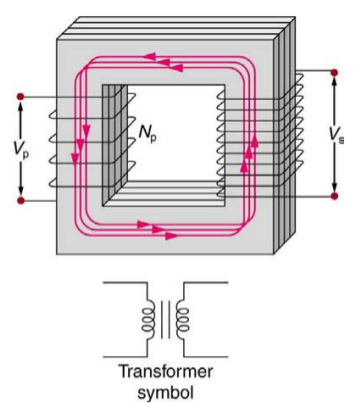
\includegraphics[width=0.35\textwidth,trim=0cm 5cm 0cm 0cm,clip=true]{figures/transformer.png}
\caption{\label{fig:trans2} The \textit{transformer} changes AC voltage levels.}
\end{figure}
Suppose the transformer in Fig. \ref{fig:trans2} has $N_L = 5$, $N_R = 100$, $V_L = 1$ kV (peak).  What is $V_R$ (peak), in kV?
\begin{itemize}
\item A: 20 kV
\item B: 5 kV
\item C: 0.05 kV
\item D: 0.05 V
\end{itemize}
\end{frame}

\begin{frame}{Motional EMF, Generators, and Transformers}
\begin{figure}
\centering
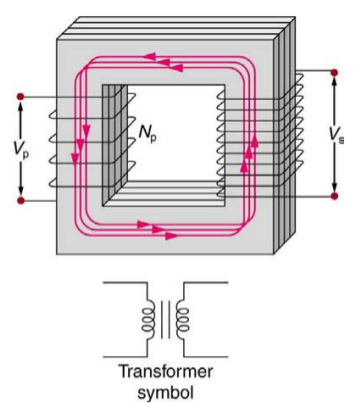
\includegraphics[width=0.35\textwidth,trim=0cm 5cm 0cm 0cm,clip=true]{figures/transformer.png}
\caption{\label{fig:trans3} The \textit{transformer} changes AC voltage levels.}
\end{figure}
\footnotesize
Suppose we need the transformer in Fig. \ref{fig:trans3} to produce $V_R = 120$ V, and $V_L = 12$ kV.  Which combination of coils will satisfy the requirement?
\begin{itemize}
\item A: $N_L = 3$, $N_R = 10$
\item B: $N_L = 10$, $N_R = 1000$
\item C: $N_L = 10$, $N_R = 100$
\item D: $N_L = 1000$, $N_R = 10$
\end{itemize}
\end{frame}

\begin{frame}{Motional EMF, Generators, and Transformers}
\footnotesize
\begin{figure}
\centering
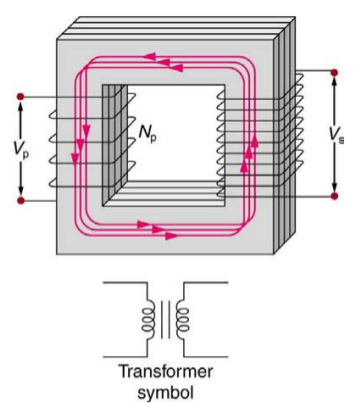
\includegraphics[width=0.25\textwidth,trim=0cm 5cm 0cm 0cm,clip=true]{figures/transformer.png}
\caption{\label{fig:trans4} \footnotesize The \textit{transformer} changes AC voltage levels.}
\end{figure}
If the $V_L \neq V_R$, how are energy and power conserved?
\begin{itemize}
\item A: The induced current is larger on the right.
\item B: The induced current is smaller on the right.
\item C: The induced current is conserved from left to right.
\item D: The induced emf is conserved from left to right.
\end{itemize}
\footnotesize
\textit{Demonstrate on board how power is conserved by (a) deriving the currents $I_L$ and $I_R$, then forming the powers $P_L$ and $P_R$.}
\end{frame}

\section{Inductors}

\begin{frame}{Inductors}
Between the coils in the transformer in Fig. \ref{fig:trans3}, there is \textit{mutual inductance:}
\begin{align}
\epsilon_L = -M \frac{\Delta I}{\Delta t}
\end{align}
\end{frame}

\section{Conclusion}

\begin{frame}{Summary}
\begin{enumerate}
\item Magnetic induction - \textbf{Chapters 23.1 - 23.5, 23.7, 23.9}
\begin{itemize}
\item Induced EMF and magnetic flux
\item Faraday's Law
\item Motional EMF, generators, and transformers
\end{itemize}
\item AC circuits - \textbf{Chapters 23.9 - 23.12}
\begin{itemize}
\item Inductors
\item RL circuits
\item RLC circuits
\end{itemize}
\end{enumerate}
\end{frame}

\end{document}
